\documentclass[journal]{IEEEtran} % use the `journal` option for ITherm conference style
\IEEEoverridecommandlockouts
% The preceding line is only needed to identify funding in the first footnote. If that is unneeded, please comment it out.
\usepackage{hyperref}
\usepackage{cite}
\usepackage{amsmath,amssymb,amsfonts}
\usepackage{algorithmic}
\usepackage{graphicx}
\usepackage{textcomp}
\usepackage{xcolor}
\def\BibTeX{{\rm B\kern-.05em{\sc i\kern-.025em b}\kern-.08em
    T\kern-.1667em\lower.7ex\hbox{E}\kern-.125emX}}
\begin{document}

\title{Predicting the duration of Invasive Mechanical Ventilation for patients in Intensive Care Unit diagnosed with Pneumonia\\}

\author{%%%% author names
    \IEEEauthorblockN{João Carvalho}% first author
    % duplicate the line above as many times as needed to list all authors
    \\%%%% author affiliations
    \IEEEauthorblockA{\textit{DETI, Universidade de Aveiro}}\\% first affiliation
    \IEEEauthorblockA{\textit{Fundamentos de Aprendizagem Automática}}\\% delete this line if not needed
    % duplicate the line above as many times as needed to list all affiliations
    %%%% corresponding author contact details
    \IEEEauthorblockA{Prof. Petia Georgieva}
}

\maketitle

\begin{abstract}
The goal of this project is to apply machine learning (ML) algorithms in order to solve a specific data science problem. In this case, the purpose is to use supervised techniques to predict the duration of Invasive Mechanical Ventilation(IMV) of patients in Intensive Care Unit(ICU) diagnosed with pneumonia. IMV can be defined as method of mechanical ventilation by establishing an artificial airway through endotracheal intubation or tracheotomy. The data was collected in the scope of a broader project that results from a scientific partnership between \hyperlink{https://ritain.io}{Ritain.io} and the Institute of Electronics and Informatics Engineering of Aveiro, \hyperlink{http://www.ieeta.pt/}{IEETA} at University of Aveiro. This is a regression problem and, based on that, four ML models were implemented and evaluated: a Deep Learning model, an Artificial neural network model, a Random Forest model and a Linear Regression model. The best result was obtained by the Random Forest which presents the best evaluation metrics(R2=0.03). This kind of predictive analysis is a great help to the hospital resource management and valuable for supporting decisions of healthcare professionals.
\end{abstract}

\begin{IEEEkeywords}
    machine learning, regression, healthcare, invasive mechanical ventilation
\end{IEEEkeywords}

\section{Introduction}
Technology and healthcare are concepts that have been increasingly working together. Over the centuries, medicine practice has benefit from several technological advancements in the various fields of healthcare and patient care, but few have had the widespread impact or influence that digital technology has. Technology solutions are assisting medical professionals as well as executive managers in improving performance, enhancing system-wide cooperation, and managing costs as the healthcare sector faces new challenges.

One of the concepts whose association with healthcare has been growing is Artificial Intelligence (AI), specifically, Machine Learning (ML). ML is a type of AI that allows software applications to become more accurate at predicting outcomes. ML algorithms use historical data as input to predict new output values. This sub-field of AI is growing in importance due to increasingly enormous volumes and variety of data. There are a large number of use cases that ML can be applied to in order to cut costs, reduce risks, and improve overall quality of life \cite{SearchEnterpriseAI2022}. Currently, a lot of attempts are being made to employ ML in healthcare, with a particular emphasis on supporting clinical decisions and getting valuable information from massive data sets. ML technologies can sort through the massive and complicated data sets produced by records, photos, sensors, and devices to uncover patterns that might enhance patient care and assist researchers in creating more effective therapies for diseases \cite{IBM}. Using ML for healthcare can open up a world of possibilities in this field e.g. improving diagnosis, developing new treatments, reducing costs and it enables to frees up healthcare providers’ time to focus on patient care rather than searching or entering information \cite{JAVAID202258}.

The goal of this project is to apply suitable ML algorithms to solve a specific data science problem, in this particular case, the purpose is to use supervised techniques to predict the duration of Invasive Mechanical Ventilation(IMV) of patients in Intensive Care Unit(ICU) diagnosed with pneumonia. IMV i.e. the method of Mechanical Ventilation(MV) by establishing an artificial airway through endotracheal intubation or tracheotomy \cite{Wang2023}. The management of MV/IMV is a crucial subject for doctors and other healthcare professionals to comprehend and employ properly since it is required to support life in acute conditions \cite{Hickey2022}. Critically sick individuals frequently require mechanical breathing for varying lengths of time and although most of these patients require ventilatory support for a short duration, approximately 30\% of them need it for more than a week \cite{Casas2015}. Intensivists routinely make predictions about the length of mechanical ventilation, especially for a "prolonged" duration, and these predictions have a significant impact on therapeutic decisions and, among these decisions, timing of tracheotomy, might be quite significant, as well as the initiation of nutrition, transfer to long-term ventilation facilities, and inclusion of patients in clinical trials \cite{Casas2015}. Besides that, timely and accurate prediction of the requirement for MV can be a significant factor to reduce patient mortality \cite{Wang2023}.

Because of all these topics, the predictive analysis of duration of IMV presents a great help to the hospital resource
management and valuable for supporting decisions of hospital
managers.

In this work, the IMV time is a continuous variable and measured in days, therefore, it will be treated as a regression problem. Four ML models will be tested to predict the LOS: a Deep Learning model, an Artificial Neural Network model, a Random Forest model and a Linear Regression model. In the next section, the practical implementation of the solution will be presented and discussed, and after that, the results and the models comparison will be analysed.

\section{State of the Art}

This section presents the bibliographic research carried out about hte IMV time prediction. Firstly the methodology of the research is detailed, then, a review of different techniques found in the literature to resolve a similar problem is presented.
\subsection{Search method}

Bibliographical research was carried out in portal \emph{Scopus} \footnote{\url{https://www.scopus.com/}}, a significant, diverse database of peer-reviewed literature.
Considering the low number of documents using machine learning
models for the prediction of IMV support time, a more embracing search were carried out with a more general term, mechanical ventilation.
Below are described the search terms used to locate relevant documents to duration of MV/IMV:

\begin{itemize}
    \item \emph{"prediction invasive mechanical ventilation duration"};
    \item \emph{"prediction mechanical ventilation duration"};
    \item \emph{"prediction mechanical ventilation duration machine learning"};
    \item \emph{"prediction invasive mechanical ventilation time pneumonia"};
    \item \emph{"prediction mechanical ventilation time pneumonia"};
    \item \emph{"invasive mechanical ventilation duration predictors"};
\end{itemize}

The figure \ref{fig:imv_docs} shows the numbers of studies by year resulting from the search terms ”prediction invasive mechanical ventilation duration”. The results demonstrate that there is a increasing demand for this topic, especially since 2017 reaching the peak in 2020, year of the rise of the corona virus disease 2019(COVID-19) pandemic in the world, a condition that have a high hospitalisation rate\cite{Nguyen2020} and may require mechanical ventilation if the patient develop acute respiratory distress syndrome (ARDS)\cite{Nakayama2022}. 

The search have included the fields “title”, “abstracts” and “keywords”, in other words, the search have only yielded documents which presents all the search terms in these three fields. The results were filtered, in the first stage, by reading the title. If the name suggests that the article has important information, then, the abstract is read carefully and the documents whose abstract had significance for the research were selected. The research was focused on the most recent articles, specifically on the last 7/8 years (from 2015 to 2022).

\begin{figure}[htp]
    \centering
    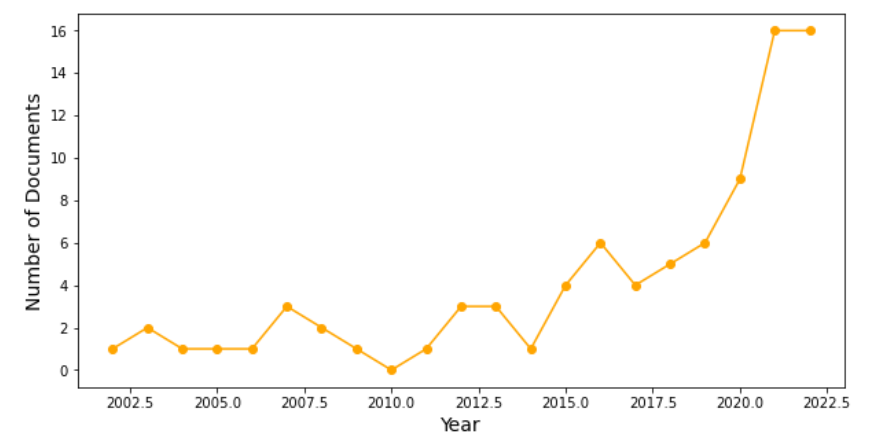
\includegraphics[width=8cm]{Project2-Report_FAA/figures/imv.png}
    \caption{Duration of IMV Prediction Documents}
    \label{fig:imv_docs}
\end{figure}


\subsection{Predicting the duration of Invasive Mechanical Ventilation (IMV)}

The table \ref{tab:papers_imv} contains the summarized information about the most relevant ML methods and results to the MV/IMV prediction found in the selected documents from the literature.

\begin{table}[]
    \centering
    \begin{tabular}{ |p{1cm}||p{3cm}|p{3cm}|  }
        \hline
        \multicolumn{3}{|c|}{Documents List} \\
        \hline
        Paper & Population & Results\\
        \hline
        \cite{Sayed2021} & Acute Respiratory Distress Syndrome Patients & -RMSE Metric: XGBoost=6.81 ± 1.18 RF=6.79 ± 1.22 LightGBM=6.41 ± 1.55
    \\
    \hline
         \cite{Figueroa-Casas2015} & Adult patients in intensive care unit & -Accuracy: LR=60\%
    \\
    \hline
        \cite{Wang2023} & Adult patients in intensive care unit & -Accuracy: LGB=0.851 RF=0.843 NN=0.856 NB=0.803 LR=0.845 SVM=0.811 KNN=0.817
    \\
    \hline
        \cite{Wang2022} & Patients with acute respiratory distress syndrome & -RMSE Metric: SVM-L= 4.39 SVM-R= 5.22 DT=5.65 RF=6.48 XGB=5.57 NN=1.59 KNN=5.57
    \\
        \hline
    \end{tabular}
    \caption{Summary of prior Studies on the Prediction duration of MV.\emph{, Logistic regression (LR), Light Gradient Boosting Machine (LGBM), Naive Bayes (NB), Support Vector Machine (SVM), Support vector Machine with Linear Kernel (SVM-L), Support Vector Machine with Radial Basis Function Kernel (SVM-R), Decision Tree (DT), Random Forest (RF), Extreme Gradient Boosting (XGB), Neural Network (NN), k-Nearest Neighbors (KNN)}}
    \label{tab:papers_imv}
\end{table}

A research of Juan B.Figueroa-Cas et al. \cite{Casas2015} intended to use machine learning techniques and statistical modeling to analyze data about the patient and their condition in order to develop a model that can accurately predict whether a patient is likely to require prolonged MV. In this study, the researchers collected data on multiple variables from the first two days of mechanical ventilation for 282 patients in a general intensive care unit. These variables and the total ventilation duration for each patient were prospectively recorded. The researchers then developed three models using different analyses to predict the duration of mechanical ventilation for these patients. The first model used multinomial logistic regression to predict whether the duration of MV would be more than 7 days, less than or equal to 7 days while the patient was alive, or less than or equal to 7 days while the patient was deceased. The second model used binary logistic regression to predict whether the duration of MV would be more than 7 days for the entire cohort and for survivors only. The third model used Cox regression to predict the time it would take for a patient to be free of mechanical ventilation while still alive. The researchers used multinomial logistic regression to develop a model that could predict the duration of MV for patients, and this model had an accuracy of 60\% (95\% confidence interval 53\%-64\%). They also used binary logistic regression to develop two models: one for the entire cohort and one for survivors only. These models had accuracies of 6\% (61\%-72\%) and 69\% (63\%-75\%), respectively.

Mohammed Sayed et al.\cite{Sayed2021} made a study which purpose was to characterize the ideal early situation during the first two days in the ICU to predict the length of MV following the start of Acute respiratory distress syndrome(ARDS) using supervised ML techniques. In this study, the researchers extracted data from the first three days in the ICU following an ARDS diagnosis for patients in the publicly available MIMIC-III database. They tracked the disease progression over these three days in order to assess lung severity according to the Berlin criteria. The researchers then used three supervised ML techniques: Light Gradient Boosting Machine (LightGBM), RF, and eXtreme Gradient Boosting (XGBoost) to predict the duration of MV for these patients. They also used the publicly available multicenter database eICU for external validation of the model. The results of this study showed that a total of 2466 and 5153 patients in the MIMIC-III and eICU databases, respectively, received MV for more than 48 hours. The median duration of MV for the extracted patients was 6.5 days in the MIMIC-III database and 5.0 days in the eICU database. The researchers found that LightGBM was the best model for predicting the duration of MV after ARDS onset in the MIMIC-III database, with a RMSE of 6.10 days. This model was also externally validated in the eICU database with an RMSE of 5.87 days.

Zichen Wang et al. \cite{Wang2022} made a study from 2022 that collected data on patients with ARDS who were admitted to ICUs. The data came from three different databases: MIMIC-IV, eICU-CRD, and AmsterdamUMCdb. The researchers used the data from the MIMIC-IV dataset to train prediction models based on seven different supervised machine learning algorithms. These models were then tested on external datasets extracted from the eICU-CRD and Amsterdamumcdb databases. The researchers also used three different machine learning explanation methods to provide an explanation for the models. The goal of this study was to develop a model that could accurately predict the duration of MV for patients with ARDS, and to provide an explanation for the model's predictions. The results of this study showed that the XGBoosting model had the most stable and accurate performance among the seven machine learning algorithms tested. This model had a root mean square error (RMSE) of 5.57 and 5.46 days in the eICU-CRD and AmsterdamUMCdb datasets, respectively. These methods showed that the use of vasopressor medication, pH level, and SOFA score had the highest effect on the prediction of MV duration for patients with ARDS.

Huiquan Wang et al. \cite{Wang2023} extracted 20 non-invasive parameters from the Medical Information Mart for Intensive Care III (MIMIC III) database. These parameters included demographic information about the patient, physiological parameters, Glasgow score, and ventilator parameters. The researchers used these data to develop a real-time early warning model of the need for IMV using seven different machine learning methods in different categories. The results of this study showed that the prediction models Lightgbm, RF, NN, NB, LR, SVM, KNN had an accuracy of 0.853, 0.843, 0.856, 0.803, 0.845, 0.811,0.817, respectively.

\section{Implementation}

This section presents the most relevant aspects regarding the data under analysis as well as the methods and their implementation details in Python.

\subsection{Data description and processing}
The data under analysis contains information of a large number of real patients admissions in ICU diagnosed with pneumonia, in Portugal.
The data was collected in the scope of a broader project that results from a scientific partnership between \hyperlink{https://ritain.io}{Ritain.io} and the Institute of Electronics and Informatics Engineering of Aveiro, \hyperlink{http://www.ieeta.pt/}{IEETA} at University of Aveiro. The data is confidential under a signed agreement between the parts and it has been properly anonymised in order to make sure that both individuals and institutions were no longer identifiable, complying with the GDPR requirements on collecting, storing and managing personal data.

The database is quite large and is comprised of a total of 83 tables. It contains 15.355 admissions in a ICU of a total of 7719 unique patients from February 02, 2009 to August 18, 2020 in about 5000 health units. Every admission has the LOS and the duration of IMV support of the patient. The tables include a variety of personal, clinical and logistic data, such as patient age, birth date, gender, vital signs, laboratory measurements, diagnoses, medications, clinical devices, types of services and more.

The selection of the relevant variables from the database was supported by a literature review carried out by Sanniya Khan Ghauri et al. \cite{Ghauri2019}. Through reading the paper, the most relevant IMV duration predictive variables were identified and, if either existing or having a similar surrogate variable in the dataset, the variable was selected and used in this analysis. The review indicated that chronic obstructive pulmonary disease and preoperative/preadmission renal impairment tends to increase IMV support time. Moreover, other factors such as the patient age, Acute Physiology and Chronic Health Evaluation (APACHE) score, ratio of arterial oxygen partial pressure to fractional inspired oxygen(PaO2/FiO2), admission type or diagnosis related group, and respiratory diseases, such as bronchitis or emphysema had a high association with the IMV time value. Additionally, Hazard et al. \cite{Hazard2020} concluded that the predicted length of ventilation for patients who were mechanically ventilated at the beginning of the example studies was longer (12.25 days for one cohort and 14.57 days for another) than it was for patients who were not ventilated after 28 days (4.34 days for one cohort and 1.41 days for another)

Therefore, this work considered the following 8 predictive variables:
\begin{itemize}
    \item "DoenteIdadeEmAnos" (age), 
    \item "TipoAdmissaoId" (admission type), 
    \item "TipoProvenienciaId" (Provenance type), 
    \item "ServicoId" (Service), 
    \item  "IntervaloAteVentilacaoInvasiva" (Time until IMV),
    \item "APACHEScore" (disease severity score), 
    \item "SAPSScore" (disease severity score), 
    \item "PaO2/FiO2 Ratio", 
    \item "DPOC" (chronic obstructive pulmonary disease), 
    \item "Insuficiência Renal" (Renal impairment), 
    \item "Enfisema" (Emphysema), 
    \item "Bonquite" (Bronchitis),
    \item "Doença do sistema respiratório" (General respiratory disease),
\end{itemize}

The dataset contains general patient's admissions, thus, it holds patients who were not submitted to IMV. For this work the dataset was filtered in order to consider only patients who was submitted to IMV. After this procedure the dataset was with 7490 admissions.

The Fig. \ref{fig:imv_box} show the distribution of the variable "IMV days" in the dataset.

\begin{figure}[htp]
    \centering
    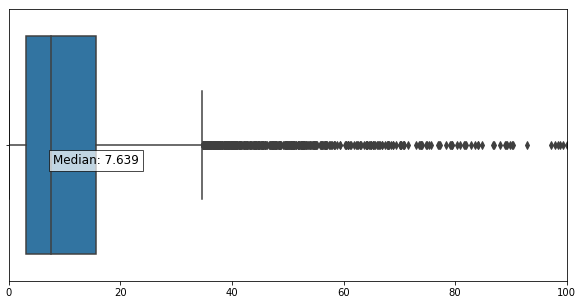
\includegraphics[width=8cm]{Project2-Report_FAA/figures/imv_box.png}
    \caption{Distribution of the "IMV support days" variable in the dataset with a mean value of 7.639 days.}
    \label{fig:imv_box}
\end{figure}

The database used to make the final dataset contains real patient's data noted and measured by healthcare professionals. The fact that this procedure was made by humans may result in a poorly measured values such as the end of ventilation support, and consequently, outliers(as may be seen, also, in the box plot \ref{fig:imv_box}). The Fig. \ref{fig:outlier} show the IMV days in all admissions and a measuring mistakes can be seen clearly. To avoid this, only IMV supports up to 1 month(30 days) were used.  After this procedure the dataset was with 6798 admissions.

\begin{figure}[htp]
    \centering
    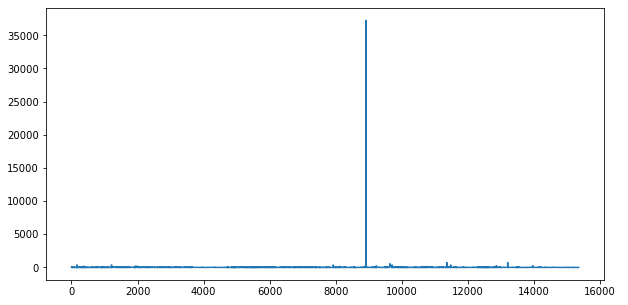
\includegraphics[width=8cm]{Project2-Report_FAA/figures/outlier.png}
    \caption{IMV days in all admissions. Axis X presents the admission and Y the number of the IMV days.}
    \label{fig:outlier}
\end{figure}

The Fig. \ref{fig:hist} presents an histogram with the distribution of the IMV days value in the filtered dataset.

\begin{figure}[htp]
    \centering
    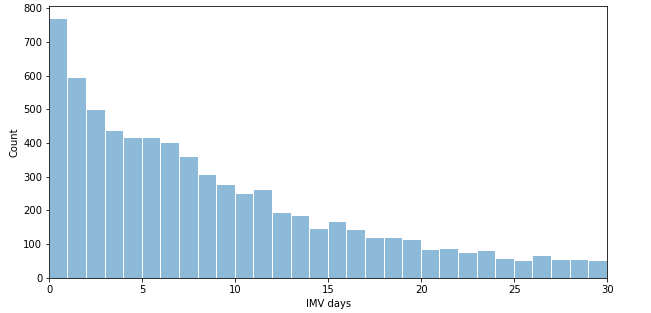
\includegraphics[width=9cm]{Project2-Report_FAA/figures/hist_imv.png}
    \caption{IMV days in all admissions. Axis X presents the admission and Y the number of the IMV days.}
    \label{fig:hist}
\end{figure}

This version of the dataset has some \textbf{missing values} in the variables: "TipoAdmissaoId", "IntervaloAteVentilacaoInvasiva DataAdmissaoHospitalar", "SAPSScore", "APACHEScore", and "PaoFioRatio". Considering that the total value of rows which have missing values(789) is small when compared with all rows, they were removed of the dataset and the final number of the dataset examples is 6009.\\

\textbf{Feature importance}

At this point it's important to analyse how much a feature is important to predict IMV. To do this a permutation feature importance analysis was carried out. Permutation feature importance is a method used in machine learning to evaluate the importance of individual features in a model's predictions. If shuffling a feature causes a significant decrease in performance, it suggests that the feature is important for the model's predictions. The model selected to make this method was random forest. The fig. \ref{fig:importance} shows the results of applying this method.

\begin{figure}[htp]
    \centering
    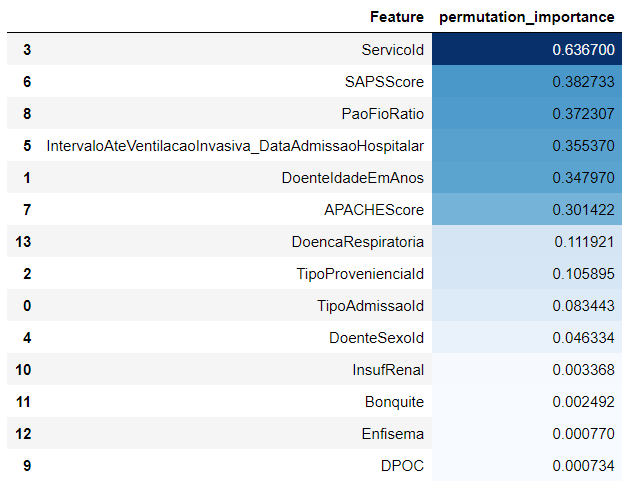
\includegraphics[width=7cm]{Project2-Report_FAA/figures/feature_sel.png}
    \caption{Permutation feature importance results.}
    \label{fig:importance}
\end{figure}

\subsection{Model training and validation}

Model validation refers to the process of evaluating a trained model with a testing data set. The main reason for using the testing dataset is to test the model's capacity to predict in the context of new data.

The validation of the models was based into two main approaches, namely Cross Validation (CV) and hyper-parameter selection (HPS). Fig. \ref{fig:cv} presents a diagram representing the overall tasks involved in the validation of a model. Briefly, the dataset is divided into a set of training data (80\% of the data) and another set of test data (20\%). The training data is used to search for an optimal model, via HPS and cross-validation, which will have a final evaluation in the test data.

\begin{figure}[htp]
    \centering
    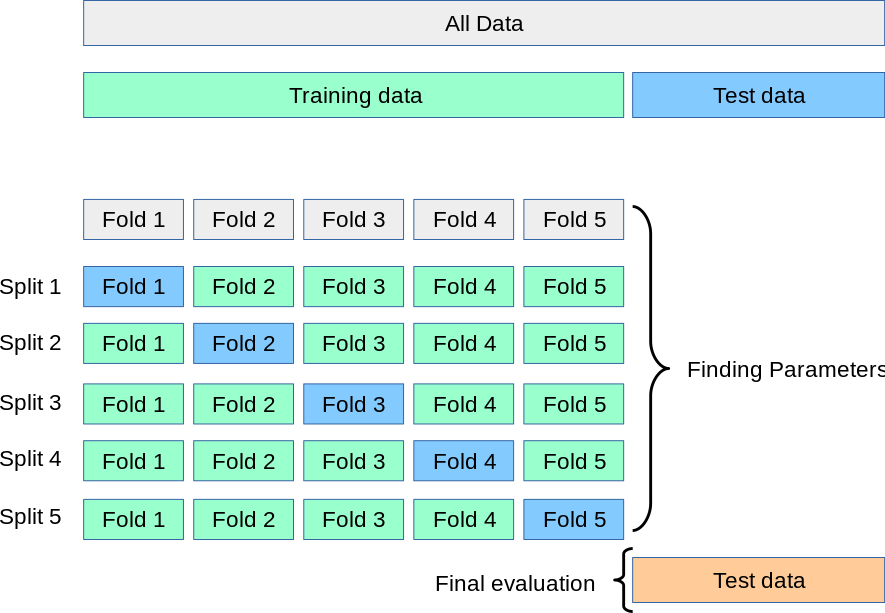
\includegraphics[width=7cm]{Project2-Report_FAA/figures/grid_search_cross_validation.png}
    \caption{Diagram fo the model validation pipeline.}
    \label{fig:cv}
\end{figure}

CV is a technique used to evaluate the performance of a machine learning model by training it on a subset of the available data and testing it on a different subset. The goal is to estimate how the model would perform on unseen data, and to identify any issues such as overfitting or underfitting. There are several types of cross-validation methods, but the most used is the k-fold cross-validation. K-fold cross-validation is a technique used to evaluate the performance of a machine learning model by dividing the data into k subsets, or "folds", of roughly equal size. The model is trained on k-1 of the folds, and tested on the remaining one. This process is then repeated k times, with a different fold being used as the test set in each iteration. The performance of the model is then averaged across the k iterations[10]. In this work 4 fold were used.

The HPS is the process of adjusting the values of the hyperparameters of a machine learning model to optimize its performance. Hyperparameters are parameters that are set before the training process and are not learned during training. It operates by doing several trials within a single training procedure. Each trial is a complete execution of the CV algorithm with values for chosen hyper-parameters. This process once finished will give the set of hyper-parameter values that are best suited for the model to give optimal results [18]. The optimal hyper-parameters were chosen by minimisation of the Mean Square Error (MSE) over the model predictions. This method of select the best combination of hyperparameters is called Grid search.

\subsection{Models}
This section includes a brief description of methods considered in this project, where the predictive models are presented in descending order complexity, namely deep learning (DL), artificial neural networks (ANN), random forest (RF) and linear regression (LR).
The \hyperlink{https://www.python.org/}{Python} implementation was based on the library \textit{Keras} (DL), the Multi-layer Perceptron regressor(MLPRegression) class from library \textit{Sklearn} (ANN), the \textit{RandomForestRegressor} class from library \textit{Sklearn} (RF) and the \textit{LinearRegression} class from \textit{Sklearn} (LR) as well as the class \textit{"Lasso"} from the library \textit{Sklearn} (LR by Lasso).\newline

\subsubsection{Deep Learning}
The development of DL models began with artificial neural networks, and it is essentially a neural network with three or more layers. A neural network with only one layer can still create approximations, but more hidden layers can help to improve and optimize for accuracy \cite{Alzubaidi2021}. DL neural networks make use of bias, weights, and data inputs to try to imitate the workings of the human brain. These elements work together to accurately recognize, classify, and describe objects within the data. One of the key features of deep learning is the use of multiple layers of artificial neurons in the network. These layers allow the network to extract features from the input data at multiple levels of abstraction, and make more complex and nuanced decisions.

Deep learning models have a number of hyperparameters that can be adjusted in order to improve their performance, such as:

\begin{itemize}
  \item \textit{'Number of layers'}: The number of layers in the deep neural network. 3 and 4 layers were tested in the model's validation and the best results was with 3 layers. 
  \item \textit{'Number of neurons'}: The number of neurons in each layer of the network. 1, 10, 30, 60, 100 and 200 were tested(same number in all layers) and the best was 200.
  %\item \textit{'Learning rate'}: The learning rate controls how quickly the model updates its weights during training. A small learning rate may lead to slow convergence, while a large learning rate can cause the model to converge too quickly and miss the optimal solution. 
  \item \textit{'Activation function'}: Activation functions are used to introduce non-linearity into the network. 'Softmax', 'softplus', 'softsign', 'relu', 'tanh', 'sigmoid', 'hard sigmoid', 'linear' were tested ad the best one was 'sigmoid'.
  \item \textit{'Batch size'}: Batch size is the number of samples used in one forward/backward pass. 10, 20, 40, 60, 80, 100 were test and the selected one was 100.
  %\item \textit{'L2 regularization'}: L2 regularization is used to prevent overfitting by adding a penalty term to the cost function that encourages the weights to be small.
  \item \textit{'Optimizer'}: Optimizer is the algorithm used to update the model's parameters during training. 'SGD', 'RMSprop', 'Adagrad', 'Adadelta', 'Adam', 'Adamax', 'Nadam' were test and the results show that the best one was 'Nadam'.

  The fig. \ref{fig:dl_h} shows the DL HPS iterations with it's optimal value.
  
\end{itemize}

\begin{figure}[htp]
    \centering
    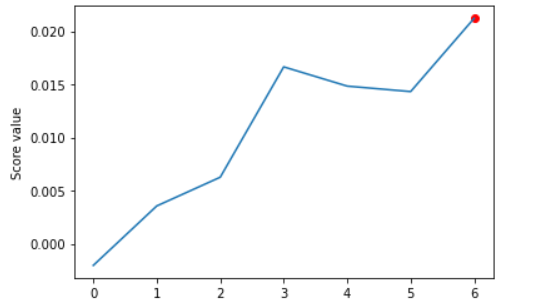
\includegraphics[width=7cm]{Project2-Report_FAA/figures/dl_hyper.png}
    \caption{DL HPS iterations for number of neurons.}
    \label{fig:dl_h}
\end{figure}

\subsubsection{Artificial neural network}
Artificial Neural Networks (ANNs) are a type of machine learning model that are inspired by the structure and function of the human brain. They are composed of interconnected "neurons" that are organized into layers. These layers are used to process and transform input data into output predictions [14]. ANNs are used in multivariate analysis to find both linear and non-linear relationships between data variables \cite{doi:10.4258/hir.2013.19.2.121}. In this project a feedforward neural networks was implemented. These networks have a specific architecture, where the information flows in one direction from the input layer to the output layer, without loops. The simplest example of this type of network is the perceptron.

The ANN's hyperparameters are similar to DL's. In this approach, the following hyperparameters were selected to be optimally tuned:
\begin{itemize}
  \item \textit{'Number of layers'}: One and two hidden layers were tested.
  \item \textit{'Number of neurons'}: This approach test 8 and 16 neurons for one hidden layer, and, (8,8), (16,16), (32,32) for two hidden layers.
  \item \textit{'Activation'}: The activation functions used were 'relu','tanh'.
  \item \textit{'Alpha'}: Strength of the L2 regularization term. The alpha values used were 0.01, 0.001, 0.0001.
  \item \textit{'Solver'}: The solver for weight optimization. The solver values used were ‘adam’ and ‘lbfgs’.
  \item \textit{'Learning rate'}: The learning rate values used were 'constant' and 'adaptive'.
\end{itemize}

After trying all combinations, the optimal hyper-parameters were: hidden layer sizes=(32, 32),  activation='tahn', alpha=0.001, solver = 'adam' and learning rate = 'constant'.

The fig. \ref{fig:ann_h} shows the ANN HPS iterations with it's optimal value.

\begin{figure}[htp]
    \centering
    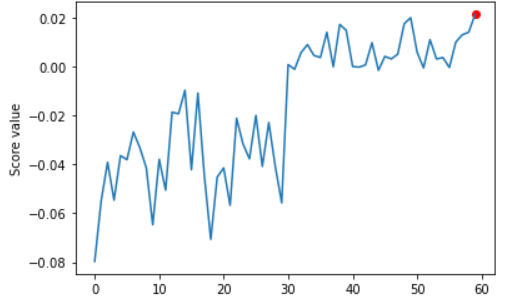
\includegraphics[width=7cm]{Project2-Report_FAA/figures/nn_hyper.png}
    \caption{ÃNN HPS iterations.}
    \label{fig:ann_h}
\end{figure}

\subsubsection{Random Forest}
RF is a type of ensemble learning method for classification and regression problems. It is a collection of decision trees, where each tree is trained on a random subset of the data. The final prediction is made by averaging the predictions of all the trees in the forest. \cite{diagnostics11122242}. The main idea behind random forest is that by combining the predictions of many decision trees, the resulting model will be more robust and have lower variance than a single decision tree. This is because each tree in the forest can make errors on a different subset of the data, and the errors will likely cancel each other out when the predictions are combined. 

Random forest has several hyperparameters that can be tuned to improve its performance, such as:
\begin{itemize}
  \item \textit{'n estimators'}: The number of trees in the forest. The values tested were 100, 200, 300 and 1000.
  \item \textit{'max depth'}: The maximum depth of the tree. The values tested were 80, 90, 100 and 110.
\end{itemize}

After trying all combinations, the optimal hyper-parameters were: n estimators=1000, max depth=110.

The fig. \ref{fig:rf_h} shows the RF HPS iterations with it's optimal value.
\begin{figure}[htp]
    \centering
    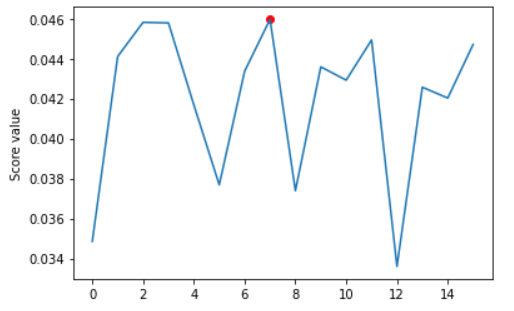
\includegraphics[width=7cm]{Project2-Report_FAA/figures/rf_hyper.png}
    \caption{RF HPS iterations.}
    \label{fig:rf_h}
\end{figure}


\subsubsection{Linear Regression}
LR is a statistical method for modeling the relationship between a dependent variable (also known as the response variable) and one or more independent variables (also known as predictors or explanatory variables). The goal of linear regression is to find the best-fitting straight line through the data points. LR models are relatively simple and provide an easy-to-understand mathematical formula that can generate predictions. In order to try to improve this method, the L1 prior as regularization technique(Lasso) was implemented with \textit{alpha} as hyper-parameter. The tested values for \textit{alpha} were 0.5, 0.05, 0.005, 0.0005, 1, 0.1, 0.01, 0.001 and 0.0001.

After trying all possible values, the optimal model were Lasso with alpha = 0.01.

The fig. \ref{fig:linear_h} shows the Lasso HPS iterations with it's optimal value.

\begin{figure}[htp]
    \centering
    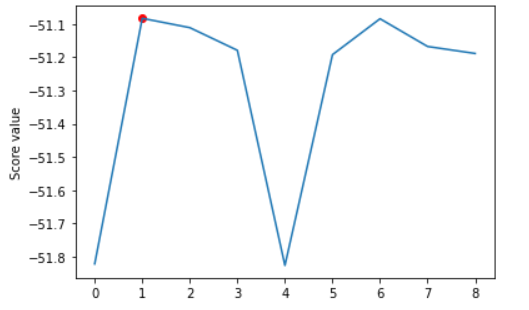
\includegraphics[width=7cm]{Project2-Report_FAA/figures/linear_hyper.png}
    \caption{Lasso HPS iterations.}
    \label{fig:linear_h}
\end{figure}

\section{Results and Discussion}
In this section the results will be analysed and discussed based on three metrics:
\begin{itemize}
  \item \textbf{R-squared(R2)}: The r2 metric (also known as the coefficient of determination) is a statistical measure that represents the proportion of the variance in the dependent variable that is explained by the independent variable(s) in a regression model. It ranges from 0 to 1(it may be bad as the model could be arbitrarily worse.), with higher values indicating a better fit of the model to the data\cite{scikit-learnR2}. 

  The R2 score is calculated mathematically as the proportion of the variance of the result y explained by the prediction $\hat{y}$ in comparison to the variance of the $\overline{y}$ mean on the test set:
  
      \[ R2 = 1 - \frac{SS(y-\hat{y})}{SS(y-\overline{y}) }\]

    where SS is the sum of squares on the test data.
    
  \item \textbf{Mean Absolute Error(MAE)}: MAE expresses the average prediction error as a percentage of the actual values. The formula for the MAE is: 

        \[ MAE = \frac{1}{n} \sum_{i=1}^{n}{ |y_i-\hat{y_i}| }\]
  
  where \textit{n} is the number of data points, $y_i$ is the actual value, and $\hat{y_i}$ is the predicted value. A value of 0\% indicates a perfect forecast, while higher values indicate a worse forecast. One of the main advantages of using the MAE is that it provides a clear and easily interpretable measure of predict error. However, it does have the disadvantage of being undefined when the actual value is zero, so it should be used with caution in these cases\cite{Myttenaere2017}.   

    
  \item \textbf{Root Mean Squared Error(RMSE)}: RMSE is calculated as the square root of the average of the squared differences between the predicted values and actual values. The smaller the RMSE value, the better the fit of the predicted values to the actual values, indicating a more accurate model.

        \[ RMSE = \sqrt{ \sum_{i=1}^{n}{ \frac{ (\hat{y_i} - y_i)^2 }{n} }}\]

 where \textit{n} is the number of data points, $y_i$ is the actual value, and $\hat{y_i}$ is the predicted value.\\
\end{itemize}

The graphics and tables below represent the results of running the models with the optimal hyper-parameters described in the section II.B.\\


\begin{figure}[htp]
    \centering
    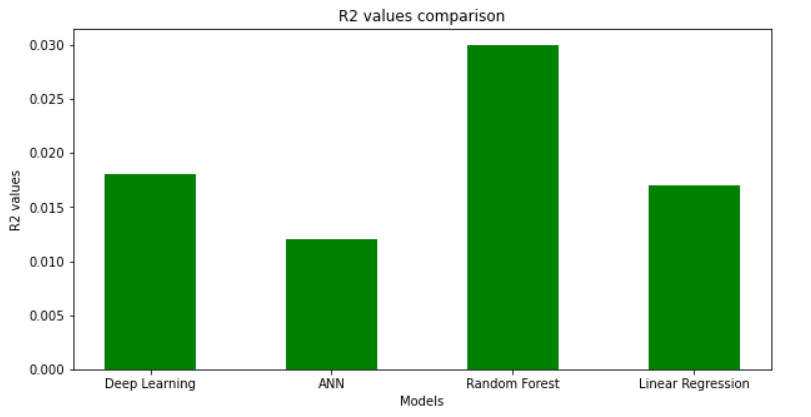
\includegraphics[width=7cm]{Project2-Report_FAA/figures/R2.png}
    \caption{R2 metric evaluation.}
    \label{fig:importance}
\end{figure}

\begin{figure}[htp]
    \centering
    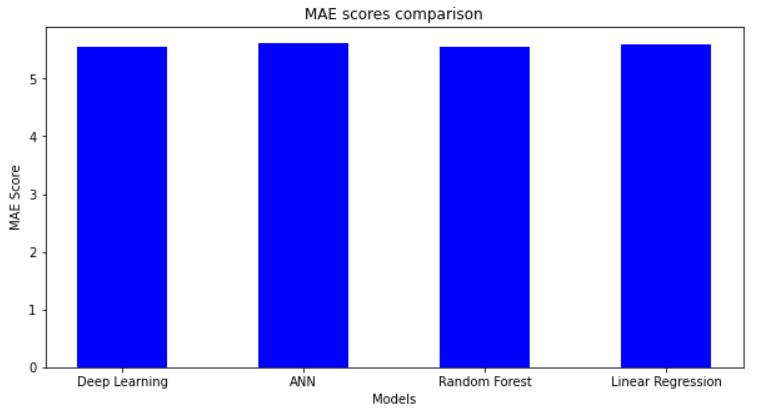
\includegraphics[width=7cm]{Project2-Report_FAA/figures/MAE.png}
    \caption{MAE metric evaluation.}
    \label{fig:importance}
\end{figure}

\begin{figure}[htp]
    \centering
    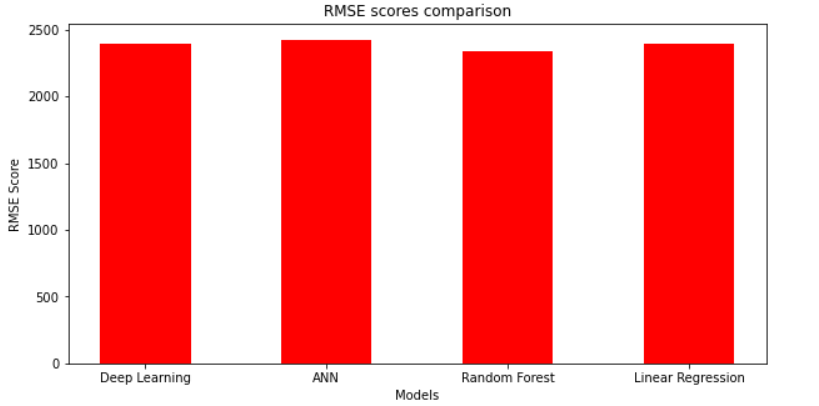
\includegraphics[width=7cm]{Project2-Report_FAA/figures/RMSE_res.png}
    \caption{RMSE metric evaluation.}
    \label{fig:importance}
\end{figure}

\begin{figure}[htp]
    \centering
    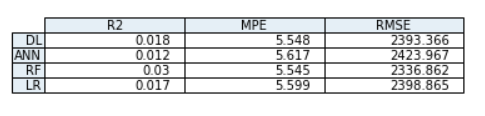
\includegraphics[width=7cm]{Project2-Report_FAA/figures/final_table.png}
    \caption{Table summarizing all results.}
    \label{fig:importance}
\end{figure}

Observing the graphics and the table in particular, we may see that the results of the models are relatively bad. The R2 values are all below 0.2 which implies a bad performance of the models. The MAE and RMSE values are also too big, especially when they are compared with the results explored in the literature. This can be explained by the fact that the features extracted are based in the very embracing
 literature research(i.e the studies were mostly about generic mechanical ventilation and dealing with the several types of patients, not only pneumonia). Additionally the database used in this work is very huge and was the first attempt to solve this problem with it. The results in the first work(predicting length of stay) were much better, that happened because this work is about a more specific topic and that fact implies a lower quality research and extraction of significant variables.

\section{Conclusion}
The development of the ML field has created new exciting possibilities for the use of ML in several areas, including healthcare. In this work, a ML approach was applied to estimate the IMV of patients in ICU diagnosed with pneumonia. Four models were implemented, validated and evaluated using three relevant metrics for regression problems. The RF model got the best results with a R2 score of 0.03. However, the models performed  relatively bad. Analysing the research table \ref{tab:papers_imv}, mainly the metric RMSE, the values in this work are much bigger. 
The large size of the database, the comprehensive research and the few number of features can explain the bad results. The DL model, for example, would have a better performance if there were more features in the final dataset considering that this kind of model is useful in cases with huge datasets.
For future work, it would be interesting to make a deeper analysis into the dataset variables in order to try to improve the model performance.

% Use this is the final version
  %  unsrt produces numbered entries, sorted by order of citation
  %  plain produces numbered entries, sorted alphabetically
  %  other styles are possible (I recommend the harvard package)
  \bibliographystyle{unsrt}
  \bibliography{Project2-Report_FAA/bibliography}% replace by the name of name of your .bib file
  

\end{document}
